\documentclass[psamsfonts]{amsart}

%-------Packages---------
\usepackage{amssymb,amsfonts}
\usepackage{enumerate}
\usepackage[margin=1.5in]{geometry}
\usepackage{amsthm}
\usepackage{theorem}
\usepackage{rotating}
\usepackage{hyperref}
\usepackage{verbatim}
\usepackage{tikz}
\usetikzlibrary{shapes,arrows}

\newenvironment{sol}{{\bfseries Solution:}}{\qedsymbol}
\newenvironment{prob}{{\bfseries Problem:}}

\bibliographystyle{plain}

\voffset = -10pt
\headheight = 0pt
\topmargin = -20pt
\textheight = 690pt

%--------Meta Data: Fill in your info------
\title{Website Changes and User Behavior \\
Using Panjiva Data to Examine Code Changes}
\date{\today}
\author{John Wang \\
14.27 Final Paper}


\begin{document}

\begin{abstract}
\end{abstract}

\maketitle

\tableofcontents

\newpage

\section{Dataset Explanation}

The proprietary Panjiva Dataset comes from the back-end databases collected by Panjiva, Inc. Panjiva's website \url{http://www.panjiva.com} acts as a medium for buyers and suppliers of manufactured goods. The site provides a communication platform so that bulk buyers of a particular good can search and obtain unbiased information on factories and suppliers of that good. These two parties can then communicate and send messages over Panjiva's interface, attempting to strike a deal. 

Panjiva's competitive advantage rests in its ability to parse government import and export data in order to obtain unbiased information about suppliers. Panjiva determines a supplier reliability score and also provides recent history of a supplier's shipments, and allows buyers to search and aggregate this information easily. Most firms that use Panjiva are large to medium size buyers of components. For example, a department store would use Panjiva to search for suppliers of shirts or clothing, or a home improvement store would search for suppliers of socket wrenches. In addition, Panjiva provides data on trends in global manufacturing and shipping by leveraging the government data it already mines for individual supplier information.

The dataset used in this paper comes from the event and activity logs of Panjiva's website. Each time a user performs some significant event or activity on the Panjiva website, an entry will be created in either the event or activity log. If the user has a registered account with Panjiva, the action will be recorded in the activity logs. All activities, regardless of whether a user has an account, are recorded in the event logs. All nontrivial features of the website, including supplier search, U.S. import and export search, and profiles views, are accounted for and stored in a SQL database.

The data in the event and activity logs are organized so that one can trace the exact user or subscribed account for which the entry. In particular, the logs contain information on the ip address of the user, the time the activity was performed, the webpage the activity occurred on, and extra data depending on the type of activity performed. 

The enormous quantity and granularity of this data enable the analysis of user-level interactions. The event logs contain about 124 million entries while the activity logs contain about 13 million entries. Moreover, the data in each of these logs extends for multiple years, allowing one to analyze the growth of Panjiva as a company and the effect of different changes to the website.

\subsection{Summary Statistics}

Summary statistics providing an overview of Panjiva's business and website are provided in table \ref{table:panjiva-overview}. Panjiva was incorporated in 2008 and has since developed a customer base composed mostly of buyers of manufactured goods. The website provides free services (a limited number of searches) for free users, and provides many more services to subscribers (there are multiple levels of subscription). 

\begin{table}[h!]
\centering
\caption{Panjiva Overview}
\begin{tabular}{l || l}
\hline
Total Users & 121,653 \\
Subscribing Users & 2,985 \\
Monthly Site Visits & 903,426 \\
Monthly Unique Visitors & 762,723 \\
Average Pages per Visit & 1.99 \\
Average Visit Duration & 1 min 18 sec \\
\hline
\end{tabular}
\label{table:panjiva-overview}
\end{table}

Commits can be thought of as changes to the code. In each commit, a software developer will introduce new code or delete old code which will then be launched to the production website. Typically a single developer at Panjiva will commit a couple of times throughout the workday. Figure \ref{fig:commit-history} shows a histogram of the number of commits throughout a 52 week period ending on 11/24/2012. Commit activity varies depending on the season and the week. In particular, commits during the summer spike upwards and there will be one or two weeks each quarter when commits fall to low levels. The second phenomenon is due to the fact that Panjiva holds a quarterly retreat where engineers reflect upon the work done over the quarter. Typically the amount of code written decreases during these weeks. 

\begin{figure}[h!]
\caption{52-Week Commit Activity}
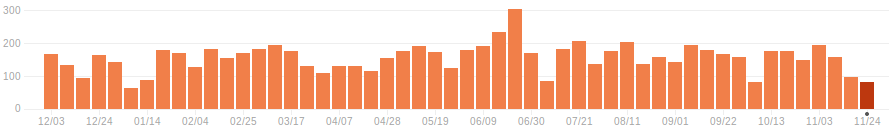
\includegraphics[width=5in]{pictures/commit-activity.png}
\label{fig:commit-history}
\end{figure}

Table \ref{table:commit-stats} shows statistics on a snapshot of the commit repository made on 11/25/2012. The table shows an enormous number of changes throughout the history of the website. In addition, the 1.3 million lines of code show that one can use the variation in the lines of code that a commit changes in order to better understand how each commit affects user behavior.

\begin{table}[h!]
\centering
\caption{Overall Commit Statistics - 11/25/2012}
\begin{tabular}{l || l }
\hline
Active Days (at least 1 commit) & 1,983 \\
Total Current Files & 20,901 \\
Total Lines of Code & 1,313,235 \\
Total Lines of Code Added & 3,989,295 \\
Total Lines of Code Removed & 2,676,060 \\
Total Commits & 29,924 \\
Total Authors/Developers & 33 \\
\hline
\end{tabular}
\label{table:commit-stats}
\end{table}

Examining commits in more detail, one can see that the majority of commits occur during working hours (from 11am to 6pm EST). Moreover, each day is fairly regular in the number of commits that occur. Commits are at a high level throughout the work day, and fall off to a low, relatively constant level throughout the night. Figure \ref{fig:commit-hours} shows the times of day during which commits happen the most frequently. 

\begin{figure}[h!]
\centering
\caption{Commit Frequency by Time of Day}
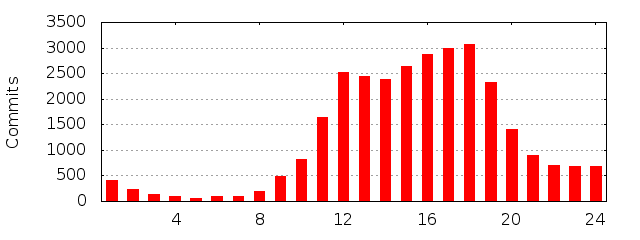
\includegraphics[width=4in]{pictures/commit-hours.png}
\label{fig:commit-hours}
\end{figure}

Finally, note that almost no commits occur on weekends. Only 5\% of the commits happen on either Saturday or Sunday.

\section{Macro-Level Results}

This section examines how code changes affect the total amount of user activity across the entire website (macro-level effects). In particular, this section analyzes the change in a number of metrics of user activity controlling for the amount of code changed in a particular day. The regression specification used will the as follows:

\begin{eqnarray}
y^i_{t} = c_0 + \bar{\gamma}^T \bar{M}_t + \bar{\beta}^T \bar{\chi}_t + \epsilon_t
\end{eqnarray}

Where $t$ indexes day, $y^i_t$ corresponds to the $i$th metric of user activity on day $t$, $\bar{M}_t$ corresponds to a vector of covariates that represent changes in the code, $\bar{\chi}_t$ is a vector of controls, and $\epsilon_t$ is an error term. We will use a number of different metrics for user activity and the specification will be run with each of them. 

The first two metrics for user actions are the total number of entries in the activity or event logs for a particular time period. Recall that event logs are database records for actions performed by anyone, while activity logs are records for only those users who have a registered account with Panjiva.

Another set of metrics are the total number of distinct users performing either activities or events in a given time period. Finally, one might also use the average number of actions per user, whether action is defined using records from activity or event logs. One would expect the each of these metrics to measure a different aspect of user behavior. 

\subsection{Daily Effects of Code Changes}

Table \ref{table:macro-action-results} displays the results from using the total action count as a metric for user activity. The regressions in table \ref{table:macro-action-results} attempt to find the effect of different changes in the code base on different measures of user activity. A commit can be measured by the number of files it changes, or the number of lines of code it changes. Changes in lines of code can be either insertions or deletions. Each of these measures is percentilized (sorted rank is divided by the total number of observations). The regressions below are performed on aggregated statistics per day, with a dummy variable equal to 1 on the weekends and 0 otherwise.  

\begin{sidewaystable}[p]
\vspace{5in}
\centering
\caption{Effect of Commits on User Activity}
{
    \def\sym#1{\ifmmode^{#1}\else\(^{#1}\)\fi}
    \begin{tabular}{l*{6}{c}}
    \hline\hline
        &\multicolumn{1}{c}{(1)}&\multicolumn{1}{c}{(2)}&\multicolumn{1}{c}{(3)}&\multicolumn{1}{c}{(4)}&\multicolumn{1}{c}{(5)}&\multicolumn{1}{c}{(6)}\\
        &\multicolumn{1}{c}{activitylogcount}&\multicolumn{1}{c}{eventlogcount}&\multicolumn{1}{c}{activitylog}&\multicolumn{1}{c}{eventlog}&\multicolumn{1}{c}{avguseractivity}&\multicolumn{1}{c}{avguserevents}\\
        &\multicolumn{1}{c}{}&\multicolumn{1}{c}{}&\multicolumn{1}{c}{distinctusercount}&\multicolumn{1}{c}{distinctusercount}&\multicolumn{1}{c}{}&\multicolumn{1}{c}{}\\
        \hline
        fileschangedpercentile&     -5530.7         &    -60589.4\sym{*}  &       460.5         &       492.7         &      -10.40\sym{*}  &      -148.6         \\
        &     (-1.91)         &     (-2.26)         &      (0.65)         &      (0.71)         &     (-2.01)         &     (-1.52)         \\
        [1em]
        insertionspercentile&      4868.8\sym{*}  &     47053.7\sym{*}  &       284.2         &       118.6         &       2.817         &       79.92         \\
        &      (2.12)         &      (2.22)         &      (0.51)         &      (0.22)         &      (0.69)         &      (1.03)         \\
        [1em]
        deletionspercentile&      2778.9         &     29970.6         &      -192.2         &      -184.4         &       4.670         &       49.47         \\
        &      (1.29)         &      (1.50)         &     (-0.36)         &     (-0.36)         &      (1.21)         &      (0.68)         \\
        [1em]
        weekend     &    -14708.0\sym{***}&    -79769.8\sym{***}&     -1060.6\sym{***}&      -816.2\sym{***}&      -0.297         &       257.0\sym{***}\\
        &    (-16.48)         &     (-9.65)         &     (-4.86)         &     (-3.82)         &     (-0.19)         &      (8.49)         \\
        [1em]
        \_cons      &     22396.6\sym{***}&    224482.8\sym{***}&      1635.7\sym{***}&      1395.9\sym{***}&       25.00\sym{***}&       340.6\sym{***}\\
        &     (25.05)         &     (27.12)         &      (7.49)         &      (6.52)         &     (15.58)         &     (11.24)         \\
        \hline
        \(N\)       &         474         &         475         &         474         &         475         &         474         &         475         \\
        \hline\hline
        \multicolumn{7}{l}{\footnotesize \textit{t} statistics in parentheses}\\
        \multicolumn{7}{l}{\footnotesize \sym{*} \(p<0.05\), \sym{**} \(p<0.01\), \sym{***} \(p<0.001\)}\\
        \multicolumn{7}{l}{The table provides regression estimates of how different measures of user actions vary with changes in the codebase.}\\
        \multicolumn{7}{l}{The table was created by aggregated data from the Panjiva activity and event logs over the period from 7/14/2011}\\
        \multicolumn{7}{l}{to 11/24/2012. Variables are broken apart by day, so that counts are per day. Activity logs record information}\\
        \multicolumn{7}{l}{about users with registered accounts, while event logs record information about all users regardless of whether they}\\
        \multicolumn{7}{l}{have registered with the Panjiva.}\\
        \\
        \multicolumn{7}{l}{Activitylogcount and eventlogcount aggregate the total number of records seen per day in the activity and event logs}\\
        \multicolumn{7}{l}{respectively. Activitylogdistincusercount and eventlogdistinctusercount aggregate the number of distinct users that}\\
        \multicolumn{7}{l}{have performed an action in either the activity or event logs respectively. Finally, avguseractivity and avguserevents}\\
        \multicolumn{7}{l}{divides the total number of records by the total number of distinct users per day to arrive at an average number of}\\
        \multicolumn{7}{l}{actions per day.}\\
        \\
        \multicolumn{7}{l}{Weekend is a dummy variable equal to 1 if the day is a Saturday or Sunday and 0 otherwise. The other covariates are}\\
        \multicolumn{7}{l}{percentilized by sorting each day and taking the rank and dividing by the total number of days. Files changed, insertions}\\
        \multicolumn{7}{l}{and deletions are obtained from commit history and are aggregated over each day. Insertions and deletions are the}\\
        \multicolumn{7}{l}{total number of lines of code inserted or deleted, respectively.}
        \end{tabular}
}
\label{table:macro-action-results}
\end{sidewaystable}

The table shows the effect of commits on same day user activity. In general, changes to the code have minor and insignificant effects on metrics derived from the event logs. There are only significant effects for the eventlogcount. However, code changes have a stronger effect on metrics derived from the activity logs. Notice that for activitylogcount, the insertionspercentile variable is significant and the fileschangedpercentile and deletionspercentile are within the 10\% significance level. Moreover, fileschangedpercentile has a significant effect on the average number of activities per user. The number of files changed and number of insertions are the only significant regressors, and they have opposing signs. 

Increasing the number of files changed tends to decrease user activity, while increasing the number of code insertions tends to increase user activity. Although this result seems perplexing, there are a number of possible explanations. First, it is possible that the commits which change fewer files tend to be higher quality commits. Thus, if a commit touches a large number of files, there is a higher likelihood that this commit would introduce a bug or contain low quality changes. However, it seems that introducing new code, instead of deleting code, has a positive effect on user activity, controlling for the number of files changed. 

Another, though possibly less satisfying explanation, is that code changes hurt average user activity in general. Since average user activity provides a measure of the organic growth of the website, it may be a better measure for the effects of code changes. Note that increasing total user count could result from a large number of new distinct user performing one or two actions each on the website. Although this could be construed as an increase in activity, each user could leave quickly, which would negatively affect long term traffic. Thus, one can think of the negative coefficient on the fileschangedpercentile variable as decreasing the long-term user activity with more code changes.

However, the second explanation seems unlikely because of the fact that code changes are constantly occuring. The regression is measuring the marginal effect of commits. Each additional file changed could provide a negative effect due to diminishing returns. Thus, one could have a negative coefficient on fileschangedpercentile even when increasing the number of files changed at very low levels (i.e. from 0 to 1) would increase user activity.

Also, notice that commits have no significant effect on the total number of distinct users. This is unsurprising since it is likely that it takes a significant period of time to increase the number of distinct users. Changes to the website will probably not spill over to other users during short time spans (like a day). Users do not have the time yet to share their new experiences on the site, so each user can be thought of as independent of others during these short time periods. Therefore, it is unsurprising that code changes fail to increase the total number of distinct users on the website. 

\subsection{Lagged Effects of Code Changes}

Note that the analysis of the previous section uses the implicit assumption that for a given day $t$, only the code changes on day $t$ influence user actions on day $t$. The previous regression assumes first that there is no lag between a code change and the change in user activity resulting from the code change, and second that only a single day's code changes affects the user activity on day $t$. Both of these assumptions are simplifications, and this section will relax the first one.

The original specification of the regression will now depend upon $y^i_{tx}$, where $x$ is a number of days of lag. Thus, if $x = 5$, then $y^i_{tx}$ will correspond to the $y^i_{t}$ which was five days ahead in the original specification. The specification will be run for all $x$ in some range $[0, R]$ to identify whether code changes have a lagged effect upon the changes in user activity. Figure \ref{fig:avg-events-time-coefficients} shows the change in the coefficients of fileschangedpercentile (in red) and lineschangedpercentile (in blue) with lags of $x \in [1, 30]$ when the regressor is average events per user from the event logs. Figure \ref{fig:avg-activities-time-coefficients} provides the same information for the regressor of average activities per user from the activity logs. 

The coefficient plotted in these figures is the $\gamma$ coefficient from the following specification (where $x$ varies from 1 to 30):
\begin{eqnarray}
y^i_{tx} = c_0 + \gamma M_{t} + \beta weekend_{t} + \epsilon_t
\end{eqnarray}

Like the previous specification, $M_t$ is a measure of code change in day $t$ (either fileschangedpercentile or lineschangedpercentile) and $weekend_t$ is a dummy variable equal to 1 if $t$ represents a day which is either Saturday or Sunday. 

Examining figure \ref{fig:avg-events-time-coefficients}, it is difficult to ascertain the actual effect of the change in time lags (note that error bars correspond to standard errors). Both covariates representing code changes, fileschangedpercentile and lineschangedpercentile, have very similar coefficients across different time lags. Small time lags less than 10 result in negative and significant coefficients for both fileschangedpercentile and lineschangedpercentile, while larger time lags tend to have positive and significant coefficients. The second trend, however, is bucked by a couple of negative coefficients when $x \in [21, 24]$. 

The amount of noise inherent in the event logs probably makes the graph difficult, if not impossible, to interpret. One could hypothesize that the shape of the curve in figure \ref{fig:avg-events-time-coefficients} suggests that code changes have differential effects depending on the amount of time lag one accounts for. However, this explanation seems week since event logs contain records of all possible users, making it difficult to interpret overall changes in the trend without decomposing into well-defined groups of users. Second, figure \ref{fig:avg-activities-time-coefficients} shows that the same results performed on the action log records provides substantially more elucidating results.

Figure \ref{fig:avg-activities-time-coefficients} shows large and consistent negative coefficients on fileschangedpercentile with all different ranges of lag. The figure also shows that the coefficient on lineschangedpercentile is not significantly different from zero for almost all lags, suggesting that it has little effect in predicting user activity. 

However, the number of files changed per day has a significant and negative coefficient throughout all time lags, reinforcing the results from the previous section that the more files changed on a particular day, the lower user activity tends to be. This result stays consistent across time, suggesting that lower user activity begins early and persists for a number of days. This provides more evidence that increasing the number of files changed per day, given the current number of files changed, will decrease user average user activity from users who are registered on Panjiva. 

Figure \ref{fig:insertions-deletions-time-coefficients} examines the change in average user activity due to insertions and deletions of code. 

\end{document}
